\documentclass[a4paper]{article}

\usepackage[margin=1in]{geometry}    
\usepackage[english]{babel}
\usepackage[utf8]{inputenc}
\usepackage[noend]{algpseudocode}
\usepackage{hyperref}
\usepackage{fancyhdr}
\usepackage{algorithm}
\usepackage{arevmath}
\usepackage{mathtools}   
\usepackage{graphicx}
\graphicspath{ {./Figures/} }  
%opening
\title{Improving Interpretability in Symbolic Regression Models Using Multi-objective GP and the Transient Terminal Set}
\author{Asher Stout, 300432820}

\begin{document}
\maketitle

%Description of initial work & hours spent
\section{Overview of Work \& Research}
\paragraph{} Work began on the project with research into previous approaches for improving the interpretability of Symbolic Regression models, and ultimately Multi-objective GP (MOGP) was selected as an area for further study. Several relevant papers defined the interpretability of a solution as the depth or size of its tree representation, which may not accurately correlate to its computational complexity. Thus, it was decided that a new measure of complexity be developed for use in MOGP. In addition, the entirely random nature of mutation operators in MOGP was identified as a place for potential innovation in improving Symbolic Regression model interpretability. This resulted in a new approach being developed called the \textbf{Transient Terminal Set}, which is described in further detail in \textbf{Section 2}.
\paragraph{} Aside from research, extensive time was invested into learning the tools required for the completion of the project objectives - particularly Python, DEAP, and LaTeX. This involved practical applications in the form of tutorials and implementing a standard MOGP and culminated in the formal definition of the Transient Terminal Set algorithm (see \textbf{Section 2}) and its implementation using DEAP (see \textbf{Section 3}). 
\paragraph{}The total hours spent on the project, as of 15 December 2020, were \textbf{135}.

%Basically the algorithm contained in TTSGP_Algorithm, with some minor formatting adjustments
\section{Transient Terminal Set}
\begin{algorithm}
	\caption{Multi-objective GP using the Transient Terminal Set (TTSGP)}
	\hspace*{\algorithmicindent} \textbf{Input:} population size \(\rho\), crossover probability \textit{p$_{c}$}, mutation probability \textit{p$_{m}$}, transient mutation probability \textit{p$_{d}$}, terminal set \(T\), function set \(F\), death age \(\alpha\) \\
	\hspace*{\algorithmicindent} \textbf{Define:} generation \(G_{n}\), individual fitness \(f_{i}\), transient terminal set \(M_{G_{n}}\), fitness threshold \(f_{t, G_{n}}\) \\ 
	\begin{algorithmic}[1]
		\State Initialize starting population \textit{$ P_{G_{0}} $}, \(M_{G_{0}}\leftarrow \emptyset\), \(f_{t, G_{0}} \leftarrow 0\)
		\While{\textit{no improvement in} \(\max f_{i}\in P_{G_{n}}\) \textit{since} \(P_{G_{n-5}}\)} \Comment{Evolve generation  \(G_{n+1}\)}
		\State \(P_{G_{n+1}}\leftarrow \emptyset\), \(M_{G_{n+1}}\leftarrow M_{G_{n}}\)
		\While{len\(P_{G_{n+1}} \neq \rho\)}	\Comment{Update population \(P_{G_{n+1}}\)}
		\State Perform crossover $\forall i\in P_{G_{n}}$ with \textit{p$_{c}$}
		\State Perform mutation $\forall i\in P_{G_{n}}$ with \textit{p$_{m}$}, \(T\), \(F\)
		\State Perform transient mutation $\forall i\in P_{G_{n}}$ with \textit{p$_{d}$, \(M_{G_{n}}\)}
		\State $P_{G_{n+1}} \leftarrow P_{G_{n+1}}\cup \{i | i_{offspring}\}$
		\EndWhile\newline
		\ForAll{subtree \(s \in  M_{G_{n+1}}\)}	\Comment{Update transient terminal set \(M_{G_{n+1}}\)}
		\If{\(age(s) > \alpha\)}
		\State Prune \(s\) from \(M_{G_{n+1}}\)
		\EndIf
		\EndFor
		\State Compute $f_{t, G_{n}}$ from $\forall f_{i} \in P_{G_{n+1}}$
		\For{$i\in P_{G_{n+1}}$}	
		\State $f_{c}\leftarrow \Delta f_{i}$ from \(G_{n}\) to \(G_{n+1}\)
		\If{ $f_{c} > $ \(f_{t, G_{n}}\)}
		\State \(M_{G_{n+1}} \leftarrow M_{G_{n+1}} \cup \{\)subtree \(s\in i \}\)
		\EndIf
		\EndFor 
		\EndWhile
\end{algorithmic}\end{algorithm}
%Provide reasoning for why the algorithm will improve interpretability
\paragraph{Note:} The transient terminal set is utilized during a genetic operation called \textit{transient mutation}, in which a candidate solution is mutated with a member of the set. The transient terminal set is composed of subtrees generated in the population (either through crossover or normal mutation) which have resulted in substantial increases in the fitness of candidate solutions.
\paragraph{} The Transient Terminal Set seeks to improve the interpretability of Symbolic Regression models via the use of multi-objective GP by improving the search process itself. By utilizing a complexity measure in addition to an error measure as the Pareto-efficient objectives for the algorithm, and pairing this with the proposed transient terminal set, it is theorized that candidate solutions will become less complex when compared with standard multi-objective GP. As the selection process for the transient terminal set follows this multi-objective framework, improvements in either objective will result in a candidate solution's altered subtree being added to the set. Thus, the transient terminal set distributes proven subtrees that result in lower errors and/or complexities throughout the population. This process potentially results in candidate solutions with both minimized error and complexity measures, and is an improvement over the entirely randomized mutation of standard multi-objective GP.

%From initial experimentation; graphs were generated using matplotlib and networkx/pygraphviz
\section{Experimentation Results}
\paragraph{Note:} The code for this experiment can be accessed at \url{https://github.com/VeryEager/transient-terminal-gp}, and the data utilized is freely accessible at \url{https://archive.ics.uci.edu/ml/datasets/wine+quality}.
\begin{figure}[H]
	\caption{Evolution using Standard GP}
	\centering
	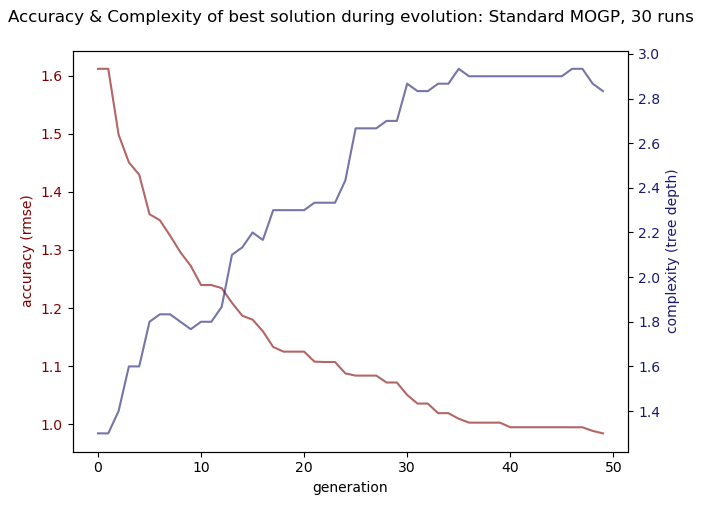
\includegraphics[width=0.5\textwidth]{Figure_1}
\end{figure}
\begin{figure}[H]
	\caption{Evolution using Transient Terminal Set GP}
	\centering
	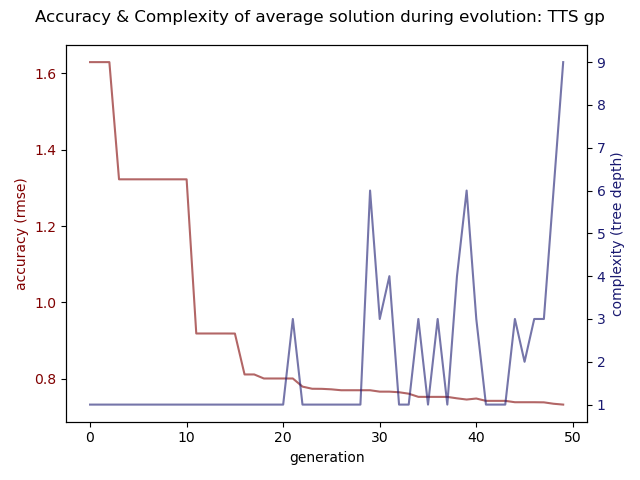
\includegraphics[width=0.5\textwidth]{Figure_3}
\end{figure}
\begin{figure}[H]
	\caption{Best individual in Standard GP Evolution}
	\centering
	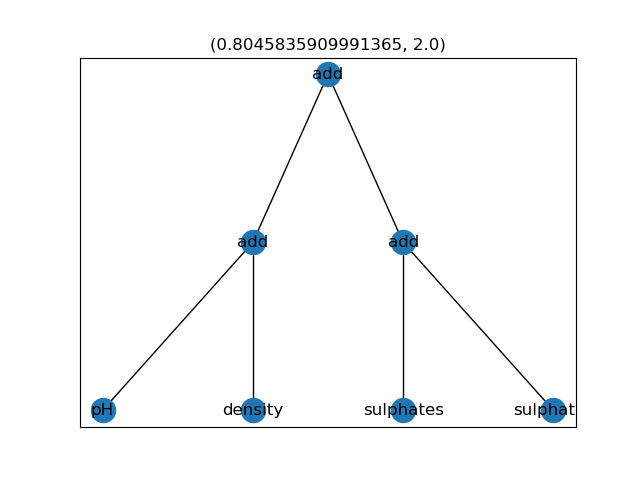
\includegraphics[width=0.6\textwidth]{Figure_2}
\end{figure}
\begin{figure}[H]
	\caption{Best individual in TTSGP Evolution}
	\centering
	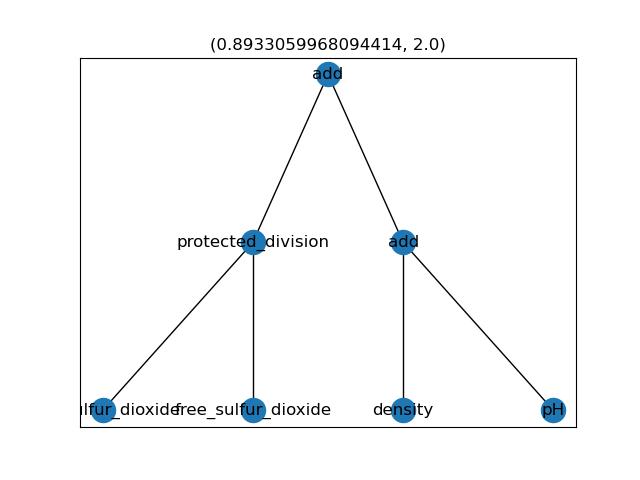
\includegraphics[width=0.9\textwidth]{Figure_4}
\end{figure}
\paragraph{} The parameters for the experiment were \textit{generations = 50}, \textit{population = 100}, \textit{crossover probability = 0.5}, \textit{mutation probability = 0.1}, and \textit{transient mutation probability = 0.05}. The results of this experiment indicate that TTSGP is competitive with standard MOGP in terms of accuracy (see \textbf{Figures 3} \textbf{4}), however does not reduce the tree depth of candidate solutions. As shown in \textbf{Figure 1} and \textbf{Figure 2}, TTSGP achieves a better accuracy in terms of rmse, however the best candidate solutions are approximately five times as complex (on average). Upon investigation I believe this behavior is caused by two factors: the selection process for members of the Transient Terminal Set, which is extremely strict and causes very few subtrees to be identified as improvements, as well as the absence of dynamic mutation probabilities for nodes in a candidate solution, which results in large subtrees being mutated deep into preexisting subtrees.

%From the ideas document
\section{Intended Future Work}
While the majority of the Transient Terminal Set algorithm has been implemented in DEAP, there are several noteworthy aspects which will be further developed or implemented to improve the results of TTSGP. \begin{itemize}
	\item First, pruning of the set will be fully implemented to ensure only relevant solutions are distributed during transient mutation.
	\item Second, the criteria for a subtree to be added to the set will be adjusted, as the mean approach is susceptible to outliers. Experimentation will be done to investigate which alternative (median, percentile, etc) is best suited for this problem.
	\item Third, as mentioned in \textbf{Section 1}, a more appropriate measure of model complexity will be created to ensure candidate solutions in TTSGP are actually less complex than those generated in standard GP.
	\item Fourth, further research and experimentation into the \textit{probability of node insertion} and \textit{probability of a terminal} during mutation will be performed, as these concepts are closely linked with the Transient Terminal Set.
	\item Fifth, various bugfixes will be performed to ensure the implementation functions as intended.
\end{itemize}

\end{document}
